
\iffalse
\begin{figure*}[ht]
    \centering
    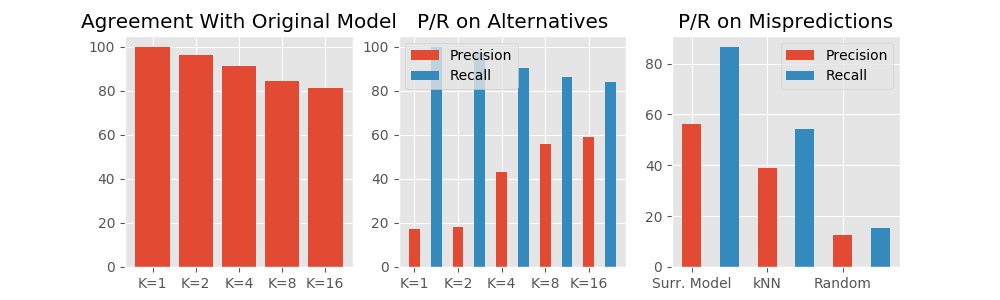
\includegraphics[width=\textwidth]{figures/result1.png}
    \caption{(A) Illustrates how well a debuggable surrogate model can approximate a complex model, (B) illustrates how well this surrogate model can isolate mispredictions in terms of precision and recall, and (C) why alternative approaches do not work.}
    \label{fig:teaser}
\end{figure*}
\fi

\section{Highlighted Results}
In this paper, we highlight some selected results to show how our hierarchical decomposition can be used to facilitate debugging. 

\subsection{Datasets}
Given a dataset, we split it into a training dataset $80\%$ and test dataset $20\%$. 

 \vspace{0.5em} \noindent \textbf{Movie: } We have a dataset of movie descriptions IMDB~\footnote{ \url{ftp://ftp.fu-berlin.de/pub/misc/movies/database/}} and Yahoo~\footnote{ \url{http://webscope.sandbox.yahoo.com/catalog.php?datatype=r}}.
Each movie has a title, a short 1-2 paragraph plot description, year, rating, language, and a list of categories, and the goal is to train a model to predict whether a movie is a ``Horror'' or ``Comedy'' from the description and title.  
The total dataset has 506,244 records.
First, using TensorFlow, we trained a LSTM-based model to predict these categories. The first layer of this model computes what is called a word-embedding, where the LSTM learns a feature-space in which similar words (co-occuring) are closer together. 
The next two layers consist of dense layers that map the words from the feature-space to classification outputs.
The result is a model that achieves 93\% accuracy, which is far more accurate than simpler alternatives on a Bag-of-Words featurization (random forests 90\%, Linear SVM 81\%, Kernel SVM 85\%).

\vspace{0.5em} \noindent  \textbf{Fraud: } ProPublica collected a dataset of corporate donations to medical researchers to analyze conflicts of interest~\cite{dollarsfordocs}. 
Records contain the PI's medical specialty, the drug brand name (null if not drug), the device brand name (null if not a device), name of pharamceutical donor, the amount donated, and whether the research is disputed.
The dataset comes with a \texttt{status} field that describes whether or not the donation was allowed under the declared research protocol.
We used a Multi-Layer Perceptron to classify disallowed donations which achieved a 82\% accuracy (random forest 81\%, Linear SVM 80\%, Kernel SVM 80\%).

\subsection{Experiments}

\begin{figure}[ht]
    \centering
    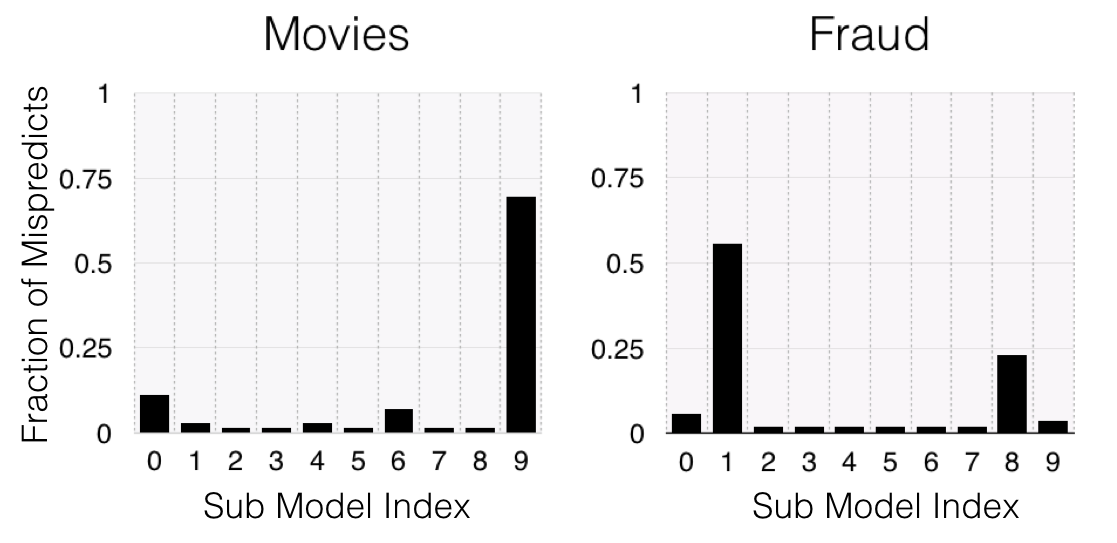
\includegraphics[width=\columnwidth]{figures/concentration.png}
    \caption{On two datasets, we show how mispredictions concentrate around specific submodels. This means there are specific regions of the feature-space most associated with mispredictions.}
    \label{fig:concentrate}
\end{figure}

\vspace{0.5em} \noindent \textbf{Exp 1. Isolating Mispredictions }  

In the first experiment, we explore whether mispredictions concentrate around particular submodels. We train the models on 80\% of the dataset, and test on the remaining 20\%. We measure the fraction of mispredictions attributed to each submodel. We want to show that mispredictions concentrate around specific submodels and are not evenly distributed throughout the feature-space. Figure \ref{fig:concentrate} shows this effect when we apply our algorithm to approximate the Movie and Fraud models with $k=10$ submodels. For the Movie dataset, 70\% of the mis-predictions are attributed to a single submodel.
For the Fraud dataset, 78\% of the errors are attributed to two of the submodels.

\begin{figure}[ht]
    \centering
    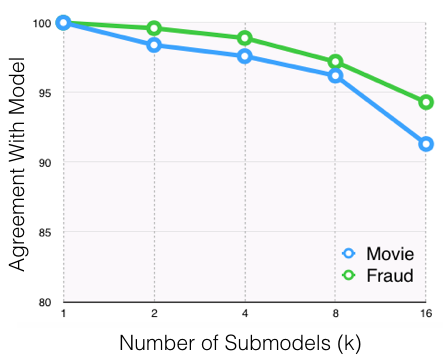
\includegraphics[width=0.6\columnwidth]{figures/agreement.png}
    \caption{On two datasets, we find that the discretized models agree with greater than 90\% accuracy with the original model. As the number of submodels increase the accuracy goes down.}
    \label{fig:agreement}
\end{figure}

\vspace{0.5em} \noindent \textbf{Exp 2. Agreement With the Original Model}
In the second experiment, we illustrate that the discretized models very accurately approximate the original model.
Figure \ref{fig:agreement} a shows the agreement between the surrogate and the original model as a function of $k$. As the model is increasingly compartmentalized with a higher $k$ the agreement goes down, however, not too drastically. The accuracy stays above 90\% for even $k=16$.


\vspace{0.5em} \noindent \textbf{Exp 3. Faster and More Accurate than Nearest Neighbors. }  
As a baseline, we compare to the following alternative approach to select possibly relevant training data to a misprediction. Given a misprediction, we find that 100 nearest neighbors in the training dataset. Since we train a decision tree meta model, we can really efficiently select the relevant data. However, nearest neighbor searches are inefficient for high-dimensional data.
For low-dimensional data, we can often use intelligent indexing structures to make this search faster (e.g., KD-Trees or Oct-Trees).
On the other hand, our approach learns a predicate with the meta-model, and the training data can be indexed w.r.t to the submodels during training time.
Our approach returns more than 20x faster than a nearest neighbor search even when coupled with dimensionality reduction and a KD-Tree.

\begin{table}[ht!]
\centering
\caption{Runtimes of the different algorithms}
\label{my-label}
\begin{tabular}{lll}
Algorithm & Movie & Fraud \\ \hline
kNN & 35.61 & 22.11  \\
kNN+PCA & 12.34 & 8.97  \\
Ours & 0.534 & 0.31 
\end{tabular}
\end{table}

However, additionally, our approach is often more accurate than the nearest neighbor approach.

\begin{table}[ht!]
\centering
\caption{Accuracy of the different algorithms}
\label{my-label}
\begin{tabular}{lllll}
Algorithm & Movie & Fraud \\ \hline
kNN & \multirow{2}{} & \multirow{2}{}  \\
kNN+PCA & \multirow{2}{} & \multirow{2}{}  \\
Ours & \multirow{2}{} & \multirow{2}{} 
\end{tabular}
\end{table}

